\section{Technische Grundlagen}
\subsection{DCF77}\label{sec_dcfgrund}
DCF77 ist ein Zeitzeichensender in Mainhausen bei Frankfurt, der seit dem ersten Januar 1959 die Uhrzeit auf der Langwellenfrequenz von 77,5 kHz sendet. Bei Sendeanlagen, die über Ländergrenzen hinaus senden, muss das Rufzeichen in der internationalen Frequenzliste eingetragen sein und das Kennzeichen des jeweiligen Landes enthalten. Deshalb wurde DCF77 gewählt, wobei das D für Deutschland steht. Der Buchstabe C war früher ein Kennzeichen für Langwelle und das F steht für Frankfurt. Da die Sendeanlage in Mainhausen mehrere Sender hat, wurde noch die Zahl 77 als Andeutung auf die Trägerfrequenz (77,5 kHz) gewählt\footnote{\cite{dcf77}, Seite 349f.}.

Das Zeitsignal wird jede Minute wiederholt und kodiert Zeit- sowie Datumsinformationen. Dabei wird jede Sekunde ein Bit übertragen. Dies geschieht durch Amplitudenmodulation. Jede Sekunde wird die Amplitude der Trägerwelle für 100 ms (logisch 0) oder 200 ms (logisch 1) auf etwa 25 \% abgesenkt. Lediglich in Sekunde 59 wird die Amplitude zur Erkennung der neuen Minute nicht abgesenkt. Tabelle \ref{tbl_dcf77kod} zeigt die Bedeutung der gesendeten Bits im DCF77-Signal\footnote{\cite{dcf77}, Seite 351ff.}.
%
\renewcommand{\arraystretch}{1}
\begin{longtable}{|l|l|}
\hline Bit & Bedeutung\\\hline\hline\endhead
\hline\endfoot\endlastfoot
%
0 & Minutenanfang\\\hline
1 - 14 & verschlüsselte Wetterinformationen\\\hline
15 & Rufbit: Ankündigung, wenn von Reserveantenne gesendet wird\\\hline
16 & A1: Wechsel von/zur Sommerzeit bei nächstem Stundenwechsel\\\hline
17 - 18 & Zeitzonenbits: 01: MEZ, 10: MESZ\\\hline
19 & A2: Schaltsekunde bei nächstem Stundenwechsel\\\hline
20 & S: Startbit (immer logisch 1)\\\hline
21 & Minutenbit, Wertigkeit 1\\\hline
22 & Minutenbit, Wertigkeit 2\\\hline
23 & Minutenbit, Wertigkeit 4\\\hline
24 & Minutenbit, Wertigkeit 8\\\hline
25 & Minutenbit, Wertigkeit 10\\\hline
26 & Minutenbit, Wertigkeit 20\\\hline
27 & Minutenbit, Wertigkeit 40\\\hline
28 & Prüfbit für Minuten, Even Parity\\\hline
29 & Stundenbit, Wertigkeit 1\\\hline
30 & Stundenbit, Wertigkeit 2\\\hline
31 & Stundenbit, Wertigkeit 4\\\hline
32 & Stundenbit, Wertigkeit 8\\\hline
33 & Stundenbit, Wertigkeit 10\\\hline
34 & Stundenbit, Wertigkeit 20\\\hline
35 & Prüfbit für Stunden, Even Parity\\\hline
36 & Kalendertag, Wertigkeit 1\\\hline
37 & Kalendertag, Wertigkeit 2\\\hline
38 & Kalendertag, Wertigkeit 4\\\hline
39 & Kalendertag, Wertigkeit 8\\\hline
40 & Kalendertag, Wertigkeit 10\\\hline
41 & Kalendertag, Wertigkeit 20\\\hline
42 & Wochentag, Wertigkeit 1\\\hline
43 & Wochentag, Wertigkeit 2\\\hline
44 & Wochentag, Wertigkeit 4\\\hline
45 & Kalendermonat, Wertigkeit 1\\\hline
46 & Kalendermonat, Wertigkeit 2\\\hline
47 & Kalendermonat, Wertigkeit 4\\\hline
48 & Kalendermonat, Wertigkeit 8\\\hline
49 & Kalendermonat, Wertigkeit 10\\\hline
50 & Kalenderjahr, Wertigkeit 1\\\hline
51 & Kalenderjahr, Wertigkeit 2\\\hline
52 & Kalenderjahr, Wertigkeit 4\\\hline
53 & Kalenderjahr, Wertigkeit 8\\\hline
54 & Kalenderjahr, Wertigkeit 10\\\hline
55 & Kalenderjahr, Wertigkeit 20\\\hline
56 & Kalenderjahr, Wertigkeit 40\\\hline
57 & Kalenderjahr, Wertigkeit 80\\\hline
58 & Prüfbit für Kalenderjahr, Even Parity\\\hline
59 & Markierung der neuen Minute, keine Amplitudenabsenkung\\\hline
\caption{Erläuterung der Bits im DCF77-Zeitsignal\footnote{\cite{dcf77}, Seite 352f.}}\label{tbl_dcf77kod}
\end{longtable}
%
\subsection{LED Matrix}
Unter LED Matrix versteht man die Ansteurung von LEDs in Zeilen und Spalten. Dabei werden alle Anoden zu Spalten und alle Kathoden zu Zeilen
verbunden. \footnote{Es kann natürlich auch die Kathode für Spalten und die
Anode für Spalten verwendet werden.} Im Vergleich zu einer einzelansteurung
bietet die LED MAatrix den großen Vorteil das bei einer Matrix $N$ Spalten
und $M$ Zeilen nur $N+M$ statt $N*M$ Leitungen verwendet werden.

\begin{wrapfigure}{r}{0.45\textwidth}
  \vspace{-25pt}
  \begin{center}
    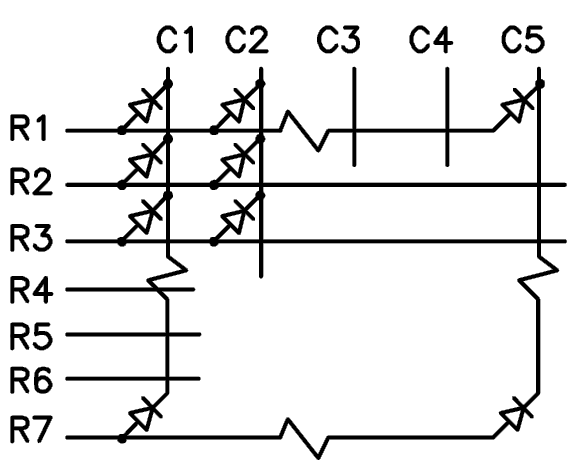
\includegraphics[width=0.42\textwidth]{skizzen/led_matrix_5x7.png}
  \end{center}
  \vspace{-20pt}
  \captionof{figure}{5x7 LED Matrix}
\end{wrapfigure}

Die LED Matrix
wird dann Zeilenweise oder Spatenweise im Multiplexbetrieb angesteuert. Das bedeutet nacheinander wird eine der Spalten mit GND versorgt und die anderen Spalten sind unbeschalten (keine Verbindung zu GND). Nun können in dieser Spalte durch anlegen von Spannung an den entsprechenden Zeilen LEDs angeschaltet werden. 
Dieser Vorgang wird für alle Spalten durchgeführt, das bedeutet es leuchten zu
einem bestimmten Zeitpunkt immer nur die LEDs einer Spalte. Durch das schnelle
umschalten zwischen den Spalten und die Trägheit des menschlichen Auge entsteht
die Illusion, dass auf der kompletten LED Matrix etwas LEDs aktiviert sind.
Als Nachteil aus dieser Beschaltung ergibt sich die veringerte Helligkeit, da
die LEDs bei $N$ Spalten nur noch $frac{1}{N}$ der Zeit leuchten können.

Der Helligkeitsverlust kann durch höheren Stromfluss zum Teil kompensiert
werden. Dass bedeutet bei $N$ Spalten werden die LEDs mit einem Pulsstrom von
$N*Nennstrom$ betrieben. Durch die Dunkelphasen kann das aktive Substrat
zwischen den Pulsen ausreichend abkühlen. Generell kann dies bis zum ca.
zehnfachen Nennstrom (200mA bei einer gewöhnlichen 20mA LED) durchgeführt
werden.\footnote{http://www.mikrocontroller.net/articles/LED-Matrix}

\subsection{Pulsweitenmodulation}\label{sec_pulsweitenmodulation}
Pulsewitenmudolation bezeichnet eine Modulationtechnik in der die Weite des
Pulse bei einer gleichbleibenden Periode verändert (siehe \ref{pwm_schma}).
Dieses Modulationstechnik erlaubt erlaube es die Leistung Geräten zu regulieren.
Der durchschnittliche Stromfluss wird durch das Verhältniss
$\frac{Pulsweite}{Periode}$ definiert. Gilt $Pulsweite=Periode$ so erhält das
Gerät 100\% der Leistung, gilt $\frac{Pulsweite}{Periode}=\frac{1}{2}$ so wird das Gerät mit halber Lesitung
versorgt.
Die Periode wird in der Regel sehr klein gewählt, zum Beispiel $\frac{1}{100}s$
bei LEDs, da das menschliche Auge 100 Hz flakern als konstantes Leuchten
wahrnimmt.
\begin{figure}[h]
  \begin{center}
    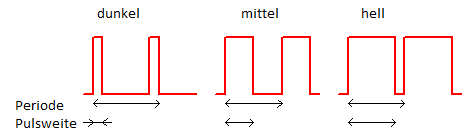
\includegraphics[width=0.8\textwidth]{skizzen/pwm.png}
  \end{center}
  \caption{Schema der Pulsweitenmodulation}
  \label{pwm_schma}
\end{figure}


